\chapter{ Технологический раздел}
\label{cha:technological}

    В данном разделе представлены средства, использованные в процессе разработки для реализации задачи, а также листинг кода программы. Кроме того показаны результаты тестирования и анализа затрачиваемой памяти.

    \section{Средства реализации}
        Для реализации поставленной задачи был использован язык C++, так как имеется большой опыт работы с ним. Для измерения процессорного времени была использована ассемблерная вставка. 


    \section{Листинг программы}
        В приведенных ниже листингах представлены следующие реализации: 
        \begin{enumerate}
            \item нерекурсивный алгоритм нахождения расстояния Левенштейна с использованием матрицы (листинг \ref{lst:matr:Levenstein1} \ref{lst:matr:Levenstein2});
            \item нерекурсивный алгоритм нахождения расстояния Дамерау-Левенштейна с использованием матрицы (листинг \ref{lst:matr:DamLevenstein1} \ref{lst:matr:DamLevenstein2});
            \item рекурсивный алгоритм нахождения расстояния Дамерау-Левенштейна (листинг \ref{lst:rec:DamLevenstein});
            \item рекурсивный алгоритм нахождения расстояния Дамерау-Левенштейна с использованием матрицы (кэшированием) (листинг \ref{lst:matr:DamLevCache1} \ref{lst:matr:DamLevCache2}).
        \end{enumerate}
        
       

        \begin{lstlisting}[language=C++, label=lst:matr:Levenstein1, caption=Функция поиска расстояния Левенштейна нерекурсивно]
        	
int Lev_Matrix(string src, string trg)
{
    if (src.length() * trg.length() == 0)
    {
        return max(trg.length(), src.length());
    }

    size_t N = src.length() + 1;
    size_t M = trg.length() + 1;

    vector<vector<int>> matrix (N);

    for (size_t i = 0; i < N; i++)
        matrix[i].resize(M);

    for (size_t i = 0; i < N; i++)
        matrix[i][0] = i;
   \end{lstlisting}
\par   \text{~~~~~~}
   \begin{lstlisting}[language=C++, label=lst:matr:Levenstein2, caption=Функция поиска расстояния Левенштейна нерекурсивно]
    for (size_t j = 0; j < M; j++)
        matrix[0][j] = j;
    
    for (size_t i = 1; i < N; i++)
    {
        for (size_t j = 1; j < M; j++)
        {
            int cost = src[i - 1] == trg[j - 1] ? 0 : 1;
            matrix[i][j] = CheckMin(matrix[i - 1][j] + 1, matrix[i][j - 1] + 1, matrix[i - 1][j - 1] + cost);
        }
    }
    return matrix[N - 1][M - 1];
}
        \end{lstlisting}
	
        \begin{lstlisting}[language=C++, label=lst:matr:DamLevenstein1, caption=Функция поиска расстояния Дамерау-Левенштейна с использованием матрицы]
        	
int DamLev_Matrix(string src, string trg)
{
    if (src.length() * trg.length() == 0)
    {
        return max(trg.length(), src.length());
    }

    size_t N = src.length() + 1;
    size_t M = trg.length() + 1;

    vector<vector<int>> matrix (N);

    for (size_t i = 0; i < N; i++)
        matrix[i].resize(M);

    for (size_t i = 0; i < N; i++)
        matrix[i][0] = i;
    
    for (size_t j = 0; j < M; j++)
        matrix[0][j] = j;
    
    for (size_t i = 1; i < N; i++)
    {
	\end{lstlisting}

\par   \text{~~~~~~}
\par   \text{~~~~~~}
\par   \text{~~~~~~}
	\begin{lstlisting}[language=C++, label=lst:matr:DamLevenstein2, caption=Функция поиска расстояния Дамерау-Левенштейна с использованием матрицы]
        for (size_t j = 1; j < M; j++)
        {
            int cost = src[i - 1] == trg[j - 1] ? 0 : 1;
            matrix[i][j] = CheckMin(matrix[i - 1][j] + 1, matrix[i][j - 1] + 1, matrix[i - 1][j - 1] + cost);
            
            if (i > 1 && j > 1 && src[i - 1] == trg[j - 2] && src[i - 2] == trg[j - 1])
                matrix[i][j] = min(matrix[i][j], matrix[i - 2][j - 2] + cost);
        }
    }
    return matrix[N - 1][M - 1];
}
        \end{lstlisting}

        \begin{lstlisting}[language=C++, label=lst:rec:DamLevenstein, caption=Функция рекурсивного поиска расстояния Дамерау-Левенштейна]
        	
static int DamLev_RecNode(string src, size_t s_len, string trg, size_t t_len)
{
    if (s_len * t_len == 0)
        return max(s_len, t_len);
    
    int cost = src[s_len - 1] == trg[t_len - 1] ? 0 : 1;

    int D = DamLev_RecNode(src, s_len - 1, trg, t_len) + 1;
    int I = DamLev_RecNode(src, s_len, trg, t_len - 1) + 1;
    int S = DamLev_RecNode(src, s_len - 1, trg, t_len - 1) + cost;

    int min_way = CheckMin(D, I, S);

    if (s_len > 1 && t_len > 1 && src[s_len - 1] == trg[t_len - 2] && src[s_len - 2] == trg[t_len - 1])
        min_way = min(min_way, DamLev_RecNode(src, s_len - 2, trg, t_len - 2) + 1);
    return min_way;
}

int DamLev_Recursion(string src, string trg)
{
    return DamLev_RecNode(src, src.length(), trg, trg.length());
}
        \end{lstlisting}
	
\par   \text{~~~~~~}

\par   \text{~~~~~~}
\par   \text{~~~~~~}
        \begin{lstlisting}[language=C++, label=lst:matr:DamLevCache1, caption=Функция рекурсивного поиска расстояния Дамерау-Левенштейна с кэшированием]
        	
static int DamLev_RecNodeWithCache(string src, size_t s_len, string trg, size_t t_len, vector<vector<int>> &matrix)
{
    if (s_len * t_len == 0)
    {
        int res = max(s_len, t_len);
        matrix[s_len][t_len] = res;
        return max(s_len, t_len);
    }
    
    int cost = src[s_len - 1] == trg[t_len - 1] ? 0 : 1;

    int D = INT_MAX;
    if (matrix[s_len - 1][t_len] == INT_MAX)
    {
        D = (DamLev_RecNodeWithCache(src, s_len - 1, trg, t_len, matrix) + 1);
    }
    else
        D = matrix[s_len - 1][t_len] + 1;
    
    int I = INT_MAX;
    if (matrix[s_len][t_len - 1] == INT_MAX)
    {
        I = (DamLev_RecNodeWithCache(src, s_len, trg, t_len - 1, matrix) + 1);
    }
    else
        I = matrix[s_len][t_len - 1] + 1;

    int S = INT_MAX;
    if (matrix[s_len - 1][t_len - 1] == INT_MAX)
    {
        S = (DamLev_RecNodeWithCache(src, s_len - 1, trg, t_len - 1, matrix) + cost);
    }
    else
        S = matrix[s_len - 1][t_len - 1] + cost;
    
    int min_way = CheckMin(D, I, S);

 \end{lstlisting}
\par   \text{~~~~~~}

\par   \text{~~~~~~}
\par   \text{~~~~~~}
\begin{lstlisting}[language=C++, label=lst:matr:DamLevCache2, caption=Функция рекурсивного поиска расстояния Дамерау-Левенштейна с кэшированием]
    if (s_len > 1 && t_len > 1 && src[s_len - 1] == trg[t_len - 2] && src[s_len - 2] == trg[t_len - 1])
    {
        int X = INT_MAX;
        if (matrix[s_len - 2][t_len - 2] == INT_MAX)
        {
            X = DamLev_RecNodeWithCache(src, s_len - 2, trg, t_len - 2, matrix) + 1;
        }
        else
            X = matrix[s_len - 2][t_len - 2] + 1;
        min_way = min(min_way, X);
    }
    if (matrix[s_len][t_len] == INT_MAX || min_way < matrix[s_len][t_len])
        matrix[s_len][t_len] = min_way;
    return min_way;
}

int DamLev_RecursionWithCache(string src, string trg)
{
    size_t N = src.length() + 1;
    size_t M = trg.length() + 1;

    vector<vector<int>> matrix (N);

    for (size_t i = 0; i < N; i++)
    {
        matrix[i].resize(M);
        for (size_t j = 0; j < M; j++)
            matrix[i][j] = INT_MAX;
    }

    int res = DamLev_RecNodeWithCache(src, src.length(), trg, trg.length(), matrix);
    return res;
}
        \end{lstlisting}
    
        
    \section{Тестирование}
        В таблице \ref{table:testing} отображён возможный набор тестов
        для тестирования методом чёрного ящика, результаты которого, 
        представленные на рисунке \ref{png:testing:result}, подтверждают
        прохождение программы перечисленных тестов.
        \begin{table}[h!]
            \caption{Тесты проверки корректности программы}
            \centering
            \begin{tabular}{|c|c|c|c|c|}
            \hline
            № & строка 1 & строка 2 & \begin{tabular}[c]{@{}c@{}}Ожидаемый результат \\ (Л, Д-Л)\end{tabular} & \begin{tabular}[c]{@{}c@{}}Фактический результат\end{tabular} \\ \hline
            1 & "скат"      & "скат"      & 0, 0                                           								 &0, 0
                                                                                      \\ \hline
            2 & "кот"        & "скат"       & 2, 2                                                                        & 2, 2                                                                         \\ \hline
            3 & "скат"     & "скат"     & 0, 0                                                                        & 0, 0                                                                         \\ \hline
            4 & "скат"     & "сакт"     & 2, 1                                                                        & 2, 1                                                                         \\ \hline
            \end{tabular}
            \label{table:testing}
        \end{table}

        \begin{figure}[h!]
            \centering
            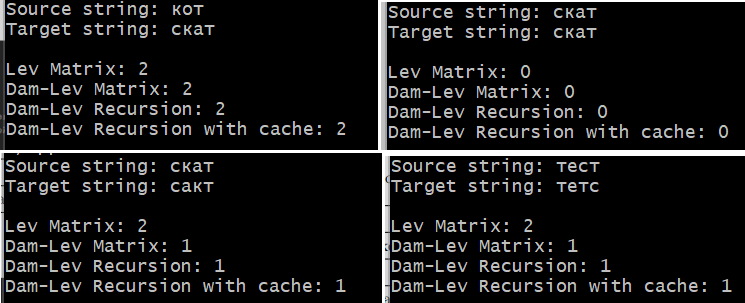
\includegraphics[scale=1]{testing.png}
            \caption{Результаты тестирования}
            \label{png:testing:result}
        \end{figure}

    \section{Сравнительный анализ потребляемой памяти}  
        Аналитически посчитаем затрачиваемую память на строках $s_1$, $s_2$ длиной n и m соответственно. Так как, с точки зрения памяти алгоритмы Левенштейна и Дамерау-Левенштейна не отличаются, достаточно рассмотреть лишь разные реализации данных алгоритмов.
        
        Использование памяти для матричного алгоритма теоритически определяется формулой (\ref{formula:memory:matr}):
        \begin{equation}
            V = 2(n+1)sizeof(int) + 2sizeof(int) + 2sizeof(size\_t) + sizeof(char)(n + m)
            \label{formula:memory:matr}
        \end{equation}
    	Где:
    	\begin{enumerate}
    			\item $2(n+1)sizeof(int)$ - память под две строки (замена матрицы в моей реализации);
    			\item $2sizeof(int)$ - память под размеры строк;
    			\item $2sizeof(size\_t)$ - память под итераторы;
    			\item $sizeof(char)(n + m)$ - память под сами строки как аргументы функции.
    	\end{enumerate}
        

        Использование памяти для рекурсивного алгоритма зависит от максимальной глубины стека вызовов. Так как эта величина равна сумме длин входящих строк, то теоритически определяется формулой (\ref{formula:memory:rec}):
        \begin{equation}
            V = sizeof(char)(n + m)  + (n + m)(2sizeof(char*) + 3sizeof(int))
            \label{formula:memory:rec}
        \end{equation}
        	Где:
    	\begin{enumerate}
    		\item $sizeof(char)(n + m)$ - память под аргументы функции;
    		\item $(n + m)(2sizeof(char*) + 3sizeof(int))$ - выделенные рекурсией ресурсы умноженные на максимальную глубину стека вызовов.
   	    \end{enumerate}
	
	\section*{Вывод}
	
	
	Были разработаны и протестированы спроектированные алгоритмы, приведены расчеты сравнительного анализа потребляемой памяти, а также указаны средства реализации поставленной задачи.
    	
\newpage